%%%%%%%%%%%%%%%%%%%%%%%%%%% asme2e.tex %%%%%%%%%%%%%%%%%%%%%%%%%%%%%%%
% Template for producing AMRob-format articles using LaTeX           
% Written by   Karla A. Camarillo Gómez                                             
%              Control Systems                                                                
%              Department of Mechanical Engineering                              
%              Instituto Tecnológico de Celaya                                         
%              Celaya, Gto., CP 38010                                                  
%              Tel: (461) 611-9114 (office)                                     
%              Fax: (461) 611-7979                                                         
%              Email: karla.camarillo@itcelaya.edu.mx                              
%              January, 2014                                           
% Modified: May 21, 2015 by Karla A. Camarillo                          
% Use at your own risk, send complaints to /dev/null               
%%%%%%%%%%%%%%%%%%%%%%%%%%%%%%%%%%%%%%%%%%%%%%%%%%%%%%%%%%%%%%%%%%%%%%

%%% use twocolumn and 10pt options with the amrob format
\documentclass[twocolumn,10pt]{amrob}
\usepackage[utf8]{inputenc}
\usepackage{graphicx}
\usepackage{mathtools}

\special{papersize=8.5in,11in}

%% The default is oneside, onecolumn, 10pt, final

%%% Replace here with information related to your conference
\confshortname{XVIII COMRob 2016, ISBN: En tr\'amite}
\vspace{0.5mm}
\conffullname{ XVIII Congreso Mexicano de Rob\'otica 2016\\
              Universidad Aut\'onoma de Sinaloa y Asociaci\'on Mexicana de Rob\'otica e Industria AC}

%%%%% for date in a single month, use
%\confdate{1-4}
%\confmonth{Octubre}
%%%%% for date across two months, use
\confdate{9--11 de Noviembre}
\confyear{2016}
\confcity{Mazatl\'an, Sinaloa}
\confcountry{M\'exico}

%%% Replace DETC2009/MESA-12345 with the number supplied to you 
%%% by ASME for your paper.
\papernum{XVIIICOMRob2016/ID-000}

%%% You need to remove 'DRAFT: ' in the title for the final submitted version.
\title{DRAFT: Diseño y Desarrollo de un Robot Omnidireccional enfocado en Robocup Small Size League}

%%% first author
\author{Full Name of First Author
    \affiliation{
	Area Department or Division Name\\
	Company or College Name\\
	City, State (spelled out), Zip Code\\
	Country (only if not MEXICO)\\
    Email: Email address (if available)
    }	
}

%%% second author
%%% remove the following entry for single author papers
%%% add more entries for additional authors
\author{Full Name of Second Coauthor\thanks{Address all correspondence to this author.} 
       {\tensfb }      
    \affiliation{Department or Division Name\\
	Company or College Name\\
	City, State (spelled out), Zip Code\\
	Country (only if not MEXICO)\\
	Email address (if available)
    }
}

\begin{document}
\graphicspath{ {./Figures/} }
\epstopdfsetup{outdir=./Figures/}
\maketitle    

%%%%%%%%%%%%%%%%%%%%%%%%%%%%%%%%%%%%%%%%%%%%%%%%%%%%%%%%%%%%%%%%%%%%%%
\begin{abstract}
{\it Este artículo describe el diseño de un robot movil omnidireccional para Robocup Small Size League, así como su construcción. Igualmente, se describen los algoritmos utilizados para lograr el movimiento omnidireccional así como el algoritmo de control utilizado. Se detalla la arquitectura del sistema, en el cual se utiliza ROS.}
\end{abstract}
% \\
% \\
% The spacing between abstract and the text heading is two line spaces.  The primary text heading is  boldface in all capitals, flushed left with the left margin.  The spacing between the  text and the heading is also two line spaces.

%%%%%%%%%%%%%%%%%%%%%%%%%%%%%%%%%%%%%%%%%%%%%%%%%%%%%%%%%%%%%%%%%%%%%%
\section*{INTRODUCCIÓN}
Con la finalidad de participar en Robocup, en la categoría Small Size League (SSL) es necesario contar con un robot que cumpla con las especificaciones establecidas en el reglamento F180 de la liga \cite{sslWiki}. Aunque dentro de estas reglas, se especifica si el robot debe ser omnidireccional, todos los equipos han optado por este tipo de robots al dar mayor libertad y agilidad a los movimientos dentro de la competencia. \par
Adcionalmente, el robot se puede utilizar en otros escenarios de investigación de Robótica. El diseño es modular y facilmente adaptable a otros requerimientos. \par
% Para poder participar en la competencia de Robocup Small Size League (SSL), es necesario cumplir con las especificaciones del reglamento F180 de la liga. Dentro de las características más importantes se encuentra que el robot debe caber dentro de un cilindro de 18 cm de altura por 15 cm de díametro. \par
% Adem\'as de participar en Robocup, es necesario que el robot se pueda adaptar fácilmente a otros escenarios de investigación de Robótica. \par
\section*{MARCO DE REFERENCIA}
Un robot de SSL debe caber dentro de un cilindro de 18 cm de altura por 15 cm de diámetro, siendo el diseño más eficiente (y el utilizado por todos los equipos) un robot cilíndrico con ruedas concéntricas. La liga cuenta con un sistema de visión el cual da la posición de cada robot y la pelota utilizada, para lo cual el robot debe cumplir con el \textit{patrón estandar} en la parte superior \cite{SSLrules2016}. Igualmente, es necesario contar con mecanismos para la pelota, los cuales son los encargados de mantener la pelota cerca del robot (\textit{dribbler}) y poder patear \textit{kickers}. \par

Un robot omnidireccional es aquel que puede moverse de un punto A a un punto B en línea recta mientras gira sobre su propio eje para llegar en una orientación dada \cite{rojasHist}. Para obtener un movimiento omnidireccional con un robot de ruedas concéntricas, es necesario contar con por lo menos 3 ruedas omnidireccionales colocadas con distintos ángulos de separación \cite{rojasForster06}. Un número de ruedas adicional proporciona redundancia, siendo 4 ruedas el dise\~no mas popular y el seleccionado. \par


%%%%%%%%%%%%%%%%%%%%%%%%%%%%%%%%%%%%%%%%%%%%%%%%%%%%%%%%%%%%%%%%%%%%%%
\section*{ARQUITECTURA DE CONTROL DE ROBOT OMNIDIRECCIONAL}
% \section*{CONTROLADOR}
La arquitectura propuesta se muestra en la Fig. \ref{fig:ROSGral}. Es necesario utilizar los componentes proporcionados por la Liga, específicamente la Visión. Para los distintos componentes que se implementantan se utiliza ROS. La utilización de ROS permite añadir funcionalidad al sistema de manera modular, facilitando la interacción entre diversos componentes. \par

% e requiere de un controlador central el cual tiene acceso al sistema de visión proporcionado por la liga de Robocup Small Size League. Este sistema aporta la posición del robot mediante cámaras en la parte superior de una cancha. El controlador está encargado de procesar la información de la posción del robot y realizar el cálculo de las trayectorias al lugar destino que se defina. Para realizar la comunicación entre los distintos componentes se utiliza ROS.\par
%%%%%%%%%%%%%%%% begin figure %%%%%%%%%%%%%%%%%%%
\begin{figure}
  \centering
    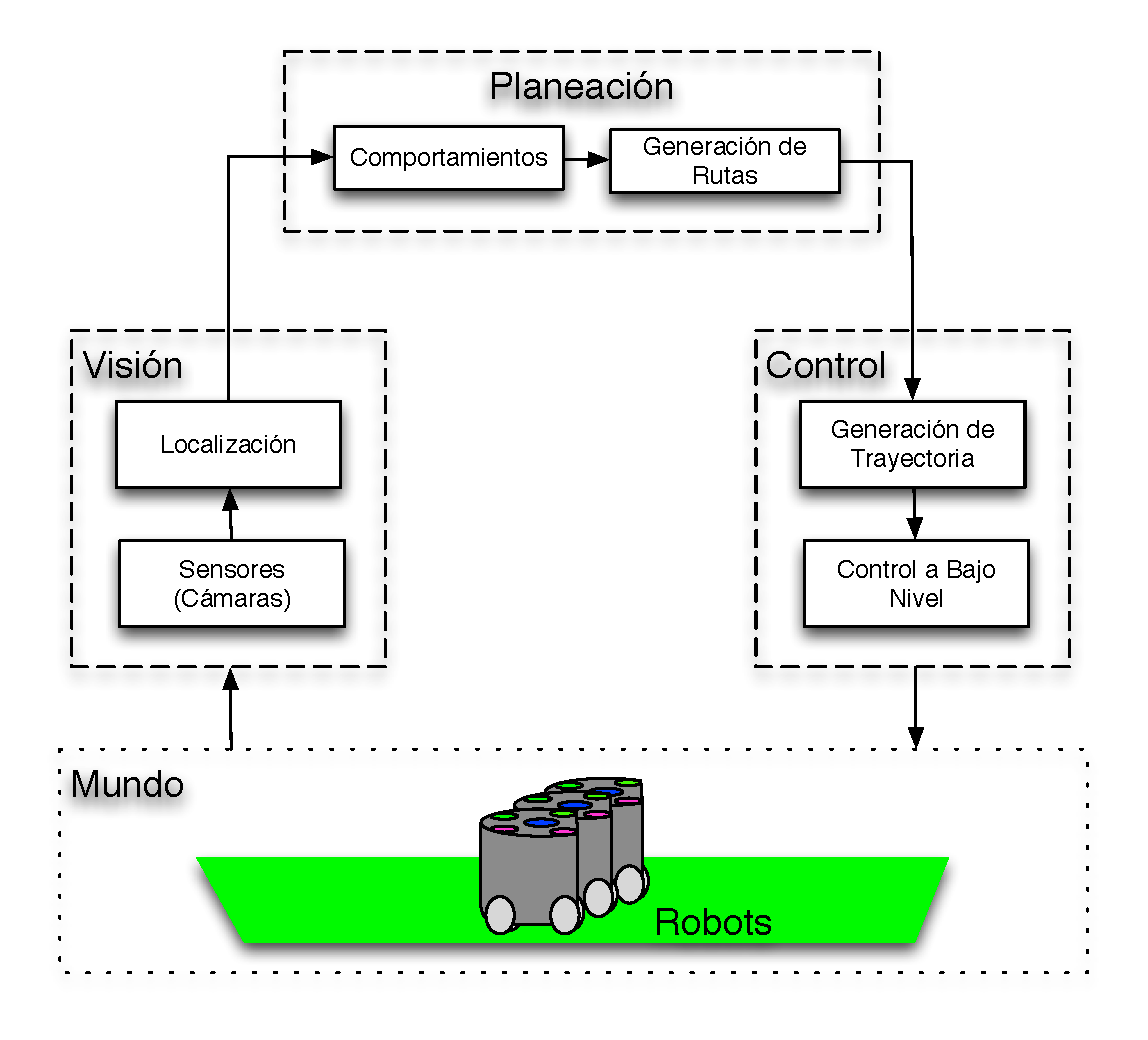
\includegraphics[width=8cm]{arqGeneral.eps}
  \caption{Diagrama del Sistema de ROS implementado}
  \label{fig:ROSGral}
\end{figure}
%%%%%%%%%%%%%%%% end figure %%%%%%%%%%%%%%%%%%% 
\subsection*{VISIÓN}
Este es un componente proporcionado por SSL. El componente utiliza las imágenes obtenidas de dos cámaras colocadas en la parte superior de la cancha, las procesa y obtiene la posición y orientación de cada robot así como la posición de la pelota. El componente no está implementando en ROS pero sus salidas son adaptadas a ROS para poder utilizarlo.
%%%%%%%%%%%%%%%%%%%%%%%%%%%%%%%%%%%%%%%%%%%%%%%%%%%%%%%%%%%%%%%%%%%%%%
\subsection*{ESTRATEGIAS}
Este componente es el encargado de realizar la planeación de tareas para todos los robots del equipo que se encuentren en el juego. Obtiene las posiciones de todos los elementos del juego de la visión así como las posiciones esperadas en un futuro de cada nodo de trayectorias.
%%%%%%%%%%%%%%%%%%%%%%%%%%%%%%%%%%%%%%%%%%%%%%%%%%%%%%%%%%%%%%%%%%%%%%
\subsection*{TRAYECTORIAS}
Cada robot cuenta con su nodo de trayectorias. Éste nodo recibe la posición actual, la deseada y el tiempo deseado del nodo de estrategias y se encarga de generar la trayectoria necesaria. De no ser posible generar la trayectoria deseada en el tiempo deseado, se reporta al nodo de Estrategias.
%%%%%%%%%%%%%%%%%%%%%%%%%%%%%%%%%%%%%%%%%%%%%%%%%%%%%%%%%%%%%%%%%%%%%%
\subsection*{COMUNICACIÓN}
Este nodo recibe la velocidad del robot deseada en cada ciclo y la envía al robot. 
%%%%%%%%%%%%%%%%%%%%%%%%%%%%%%%%%%%%%%%%%%%%%%%%%%%%%%%%%%%%%%%%%%%%%%
\section*{DISEÑO DEL ROBOT}

Realizando un análisis de los robots de la liga, se determinó que la velocidad máxima deseada del robot se estableciera en 3.5 m/s. Igualmente, la carga que el robot debe soportar se estableció en 2.5 Kg. Debido a la velocidad del juego, es común que ocurran colisiones entre ellos por lo que el exterior del robot debe ser de un material resistente además contar con piezas fácilmente reemplazables.\par

Para poder realizar numerosas pruebas de las distintas partes que conforman al robot, se optó por utilizar el modelado por deposición fundida (impresión 3D). Adicionalmente, este método permite realizar diseños más complejos además de probarlos y validarlos rápidamente. Se utilizaron dos tipos de plástico: ABS y HIPS. Se realizó un diseño modular para facilitar futuras mejoras, asi como volverlo fácilmente adaptable a otros escenarios.\par

La electrónica del robot se compone de una tarjeta de desarrollo MOJO la cual tiene una FPGA Spartan 6 XC6SLX9 y un microcontrolador ATmega32U4. Para la comunicaci\'on, se utiliza una tarjeta XBee WiFi. Para el control de los motores, se utiliza un ESC (Electronic Speed Controller) por motor. La interaccion de los componentes se muestra en \ref{fig:electGral}. \par
%%%%%%%%%%%%%%%% begin figure %%%%%%%%%%%%%%%%%%%
\begin{figure}
  \centering
    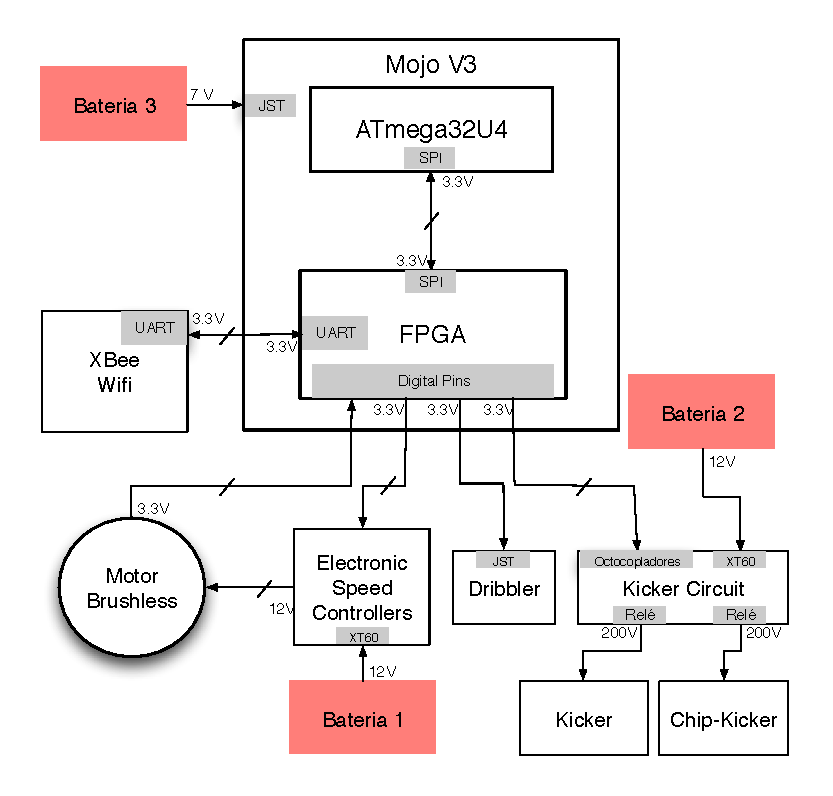
\includegraphics[width=8cm]{diagElectronica.eps}
  \caption{Componentes de Electrónica}
  \label{fig:electGral}
\end{figure}
%%%%%%%%%%%%%%%% end figure %%%%%%%%%%%%%%%%%%%
%%%%%%%%%%%%%%%%%%%%%%%%%%%%%%%%%%%%%%%%%%%%%%%%%%%%%%%%%%%%%%%%%%%%%%
\subsection*{CARCASA Y BASE}
La base es la pieza en la cual se ensamblan el resto mientras que la carcasa protege al resto del robot de posibles impactos durante su funcionamiento. Estas piezas constituyen las piezas de mayores dimensiones en el dise\~no por lo que son manufactaras usando plástico HIPS al ofrecer mejores resultados en piezas de grandes dimensiones. La carcasa est\'a formada por 4 piezas \'unicas. Como parte de la carcasa se incluye el patrón necesario para que la visi\'on de la liga proporcione la posici\'on del robot.\par
%%%%%%%%%%%%%%%%%%%%%%%%%%%%%%%%%%%%%%%%%%%%%%%%%%%%%%%%%%%%%%%%%%%%%%
\subsection*{ENERGÍA}
Los componentes que requieren de electricidad para funcionar son tres: mecanismos para el movimiento, para la pelota y el cómputo. Cada uno utiliza su propia batería LiPo para tenerlos aislados entre si, para la comunicación entre ellos se utilizan optocopladores. Los mecanismos para el movimiento, motores y ESC son alimentados por una batería de 12 V. Los mecanismos para la pelota, Kickers y dribbler, son alimentados por una batería de 12 V. El componente de cómputo es alimentado por una batería de 7 V.
%%%%%%%%%%%%%%%%%%%%%%%%%%%%%%%%%%%%%%%%%%%%%%%%%%%%%%%%%%%%%%%%%%%%%%
\subsection*{MECANISMOS PARA MOVIMIENTO DEL ROBOT}

%%%%%%%%%%%%%%%%%%%%%%%%%%%%%%%%%%%%%%%%%%%%%%%%%%%%%%%%%%%%%%%%%%%%%%
\subsubsection*{RUEDA}
La mayoria de los diseños de ruedas omnidireccionales comerciales están enfocados en aumentar la eficiencia de la rueda buscando que el perfil de la rueda se perfectamente circular (\cite{rojasHist}), sacrificando el espacio utilizado por la rueda. Debido a las reestricciones en las dimensiones del robot, se realizó un diseño propio. La rueda omnidireccional más común dentro de la liga consiste en una rueda con rodillos perpendiculares al eje principal. \par

Los factores más importantes en el diseño de la rueda es la facilidad de ser ensamblada y la resistencia del material utilizado. El diseño final utilizado utiliza cuatro piezas únicas, de las cuales 2 son de diseño propio: una pieza de plástico ABS (\ref{fig:ruedaOmni}) y 21 rodillos de aluminio; y dos piezas comerciales: 1 cable de acero y 21 orings. \par

Como solamente una pieza conforma el esqueleto de la rueda, se simplifica el ensablado además de hacer ser más resistente comparado con otras versiones que utilzan varias piezas como esqueleto. Adicionalmente, el radio de la rueda así como el número de rodillos utilizados favorece un funcionamiento efectivo de la rueda comparado con versiones de menor tamaño o menor número de rodillos.\par

%%%%%%%%%%%%%%%%%%%%%%%%%%%%%%%%%%%%%%%%%%%%%%%%%%%%%%%%%%%%%%%%%%%%%%
%%%%%%%%%%%%%%%% begin figure %%%%%%%%%%%%%%%%%%%
\begin{figure}[t]
  \centering
    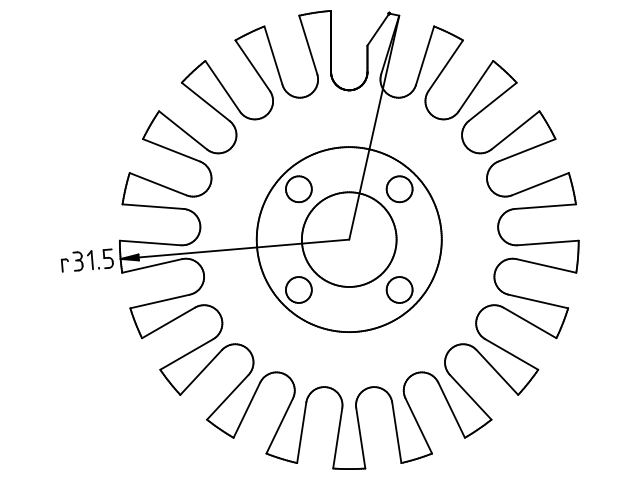
\includegraphics[width=8cm]{rueda.png}
  \caption{Diagrama de la Rueda Omnidireccional Utilizada}
  \label{fig:ruedaOmni}
\end{figure}
%%%%%%%%%%%%%%%% end figure %%%%%%%%%%%%%%%%%%% 
%%%%%%%%%%%%%%%%%%%%%%%%%%%%%%%%%%%%%%%%%%%%%%%%%%%%%%%%%%%%%%%%%%%%%%
\subsubsection*{REDUCTOR}
El motor utilizado es Maxon 200142. Este motor tiene una velocidad sin carga de 4370 RPM (nominal de 2940 RPM). Dados los requerimientos de velocidad y peso soportado del robot, es neceario utilizar un reductor de velocidad de 3.5. Se utiliza un reductor conformado por engranes cilíndricos rectos de metal. Se utilizan engranes comerciales debido a la necesidad de contar con alta eficiencia en la transmisión de la energía además de tener que ser resistentes en altas velocidades. \par
%%%%%%%%%%%%%%%%%%%%%%%%%%%%%%%%%%%%%%%%%%%%%%%%%%%%%%%%%%%%%%%%%%%%%%
\subsubsection*{ELECTRONIC SPEED CONTROLLER (ESC)}
Se utiliza un ESC por motor que sirve de interfaz entre la FPGA que envía una señal PWM y el motor. Este componente permite aisalar eléctricamente la FPGA (que utiliza voltaje TTL) de los motores (que utilizan 12V). Se utiliza un modelo de ESC dedicado a drones multihélice debido a la rapidez de respuesta que estos ofrecen y que resulta necesaria para el correcto funcionamiento de cada motor.\par 
%%%%%%%%%%%%%%%%%%%%%%%%%%%%%%%%%%%%%%%%%%%%%%%%%%%%%%%%%%%%%%%%%%%%%%
\subsection*{MECANISMOS PARA LA PELOTA}
En esta sección se presentan los mecanismos diseñados para tener control de la pelota (\textit{dribbler}) así como el mecanismo de pateo (\textit{Kicker}).
%%%%%%%%%%%%%%%%%%%%%%%%%%%%%%%%%%%%%%%%%%%%%%%%%%%%%%%%%%%%%%%%%%%%%%
%%%%%%%%%%%%%%%% begin figure %%%%%%%%%%%%%%%%%%%
\begin{figure}
  \centering
    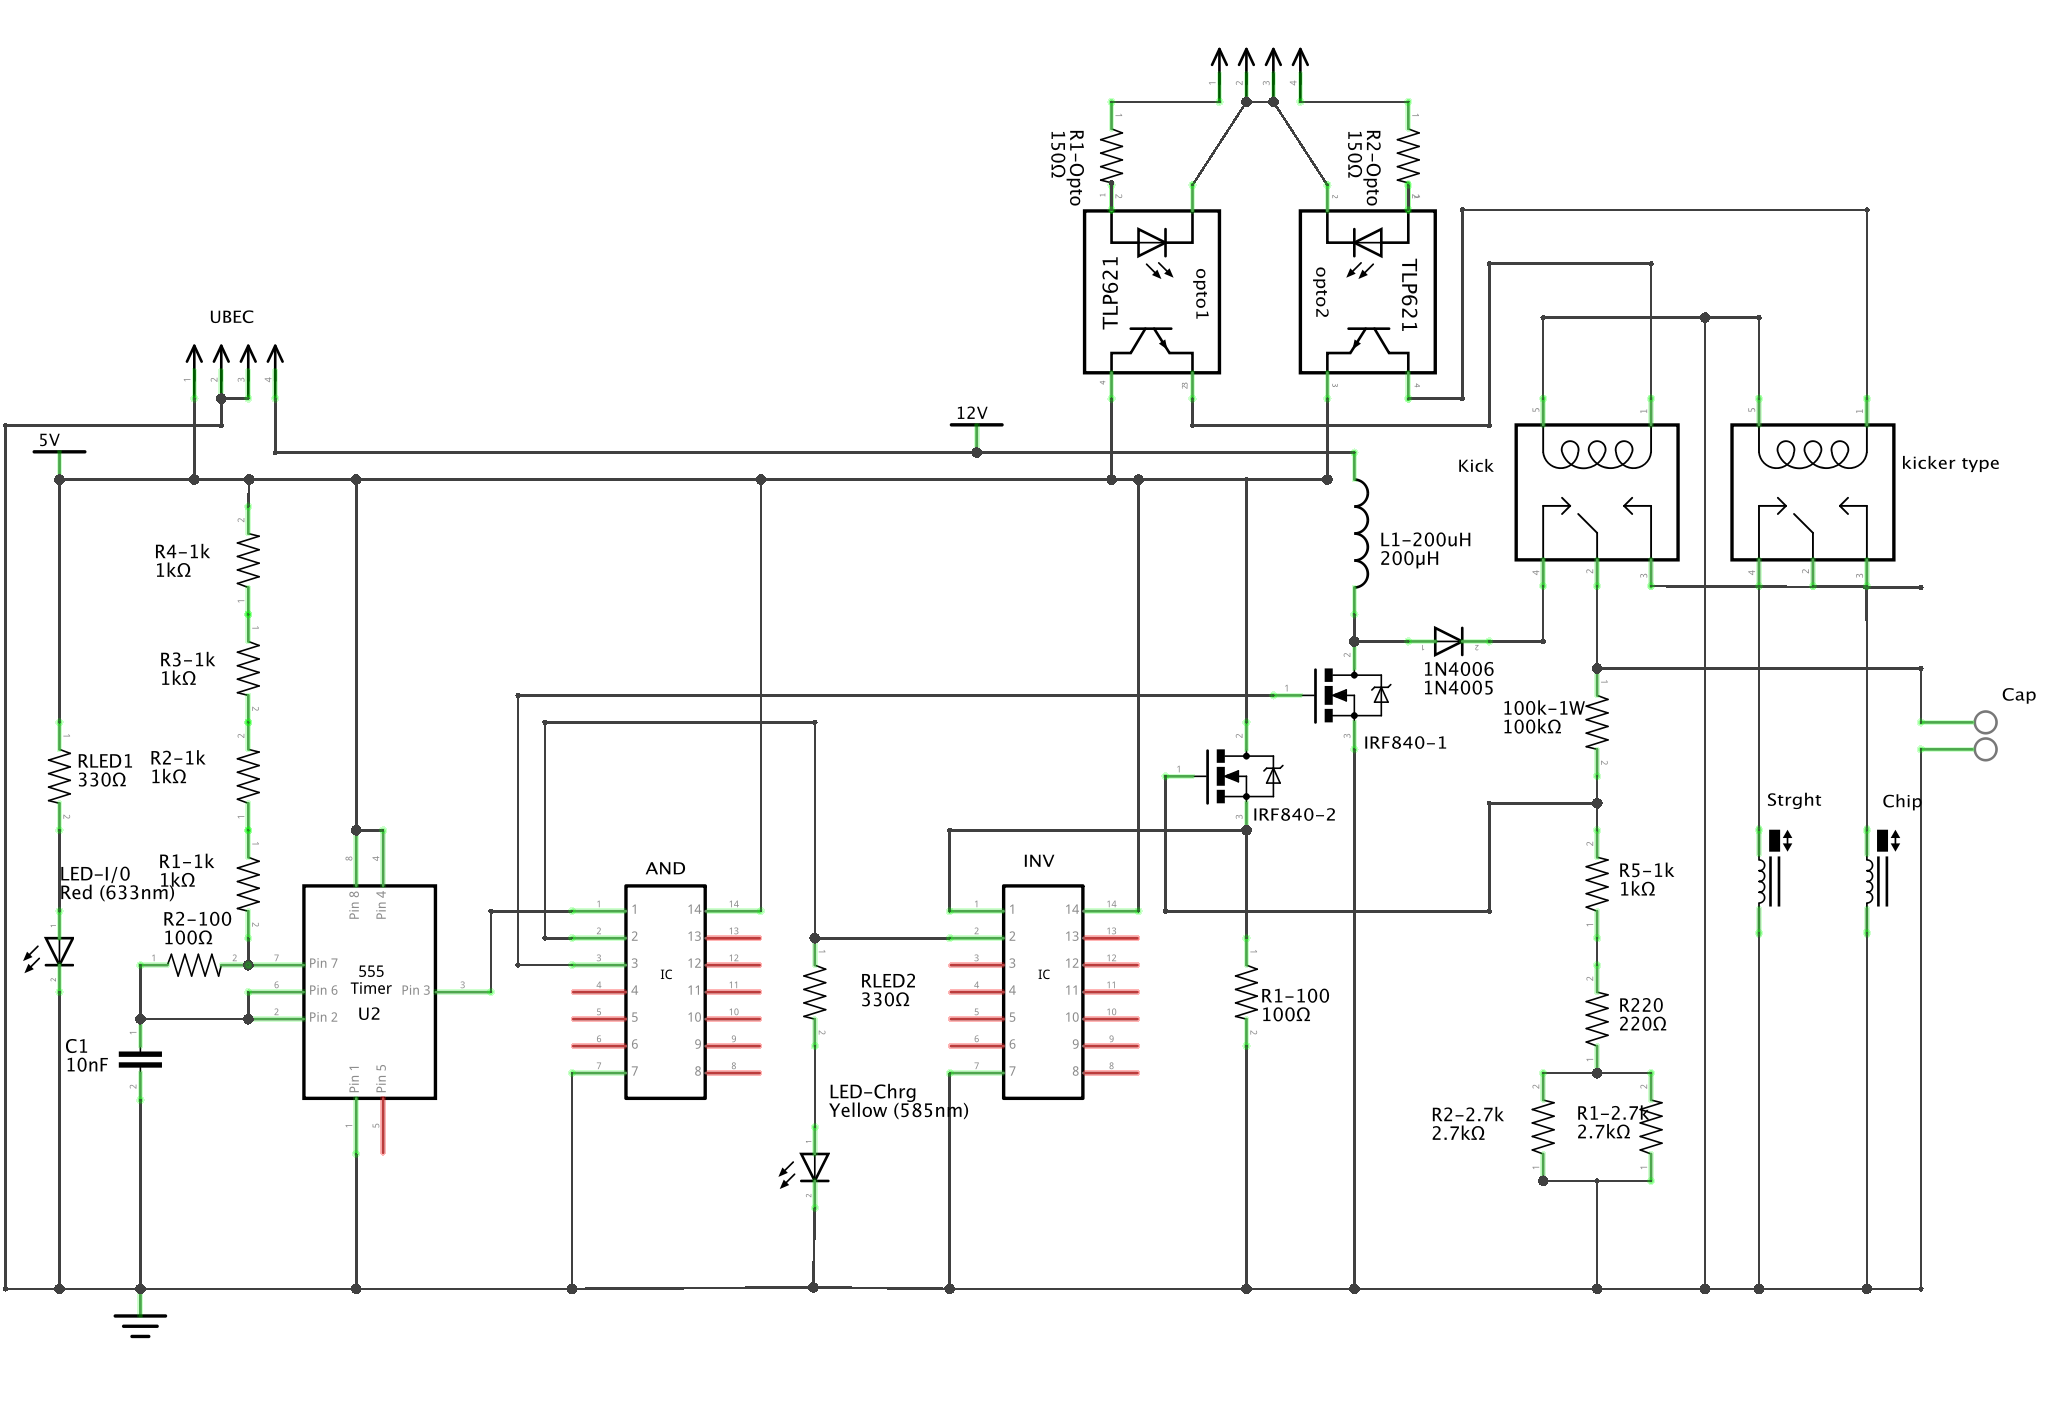
\includegraphics[width=8cm]{circuitoKicker.png}
  \caption{Circuito para el Kicker}
  \label{fig:elecKicker}
\end{figure}
%%%%%%%%%%%%%%%% end figure %%%%%%%%%%%%%%%%%%%
%%%%%%%%%%%%%%%%%%%%%%%%%%%%%%%%%%%%%%%%%%%%%%%%%%%%%%%%%%%%%%%%%%%%%%
\subsubsection*{KICKERS}
Se utiliza un seleonoide el cual es alimentado con 200 V cuando se da la señal para patear. En la Fig. \ref{fig:elecKicker} se muestra el circuito utilizado para llevar la entrada de 12 V a una salida de 200 V. Dentro del circuito, se utiliza un \textit{Universal Battery Elimination Circuit (UBEC)} para alimentar con 5 V los circuitos integrados a partir de los 12 V de la batería. \par
%%%%%%%%%%%%%%%%%%%%%%%%%%%%%%%%%%%%%%%%%%%%%%%%%%%%%%%%%%%%%%%%%%%%%%
\subsubsection*{DRIBBLER}
El mecanismo del dribbler consiste en un motor DC que funciona entre 3 y 5 V así como un sistema de engranes de plástico para la transimisión de energía y una espuma en el punto de contacto con la pelota. Para el control del dribbler se utiliza un Puente H en modo unidireccional. \par 
% Para el dribbler, se utiliza un Puente H en modo unidireccional para controlar un motor DC. \par
%%%%%%%%%%%%%%%%%%%%%%%%%%%%%%%%%%%%%%%%%%%%%%%%%%%%%%%%%%%%%%%%%%%%%%
% \subsubsection*{DRIVER}

%%%%%%%%%%%%%%%%%%%%%%%%%%%%%%%%%%%%%%%%%%%%%%%%%%%%%%%%%%%%%%%%%%%%%%
\subsection*{CÓMPUTO}
En esta sección se detallan los componentes de cómputo utilizados. Estos componentes mandan las señales necesarias a cada actuador además de recibir las señales de los sensores utilizados. Realizan los cálculos necesarios para el movimiento así como la comunicación con el resto del sistema.  
%%%%%%%%%%%%%%%%%%%%%%%%%%%%%%%%%%%%%%%%%%%%%%%%%%%%%%%%%%%%%%%%%%%%%%
\subsubsection*{FPGA}
Debido a que es necesario controlar los 4 motores así como otros componentes, es necesario contrar con la capcidad de atender múltiples entradas y salidas al mismo tiempo. Una FPGA ofrece esta capacidad además de tener mayor resolución respecto a un microcontrolador. En el sistema implementado, la FPGA tiene seis funciones:
\begin{enumerate}
  \item Recibir los datos del XBee.
  \item Calcular la velocidad de cada motor mediante la señal de cada sensor hall.
  \item Mandar la velocidad deseada a cada ESC mediante PWM.
  \item Activar el dribbler
  \item Activar el kicker
  \item Recibir y procesar la señal de sensores adicionales
\end{enumerate}
La FPGA se comunica con el Microcontrolador mediante SPI y Memory Mapping. Envía las velocidades deseadas \(X, Y y \omega\) así como las velocidades reales de cada motor y recibe las velocidades deseadas para cada motor.\par

%%%%%%%%%%%%%%%%%%%%%%%%%%%%%%%%%%%%%%%%%%%%%%%%%%%%%%%%%%%%%%%%%%%%%%
\subsubsection*{MICROCONTROLADOR}
En cada ciclo del microcontrolador, se reciben las velocidades deseadas \(X, Y y \omega\) así como las realeas de cada motor y se determina una nueva velocidad deseada de motor mediante el modelo omnidireccional así como aplicando un algoritmo de control PI. Las velocidades por motor calculadas son transferidas a la FPGA.
% En cada ciclo, se leen los registros de las velocidades de cada motor (deseada y real) y se realizan los cálculos para determinar la nueva velocidad de cada motor de acuerdo a los modelo omnidireccional y al algoritmo de control utilizado. \par

%%%%%%%%%%%%%%%%%%%%%%%%%%%%%%%%%%%%%%%%%%%%%%%%%%%%%%%%%%%%%%%%%%%%%%
\subsubsection*{COMUNICACIÓN}
Para el control del robot es necesario contar con comunicación inalámbrica (\'unicamente esta prohibido usar bluetooth). Se opt\'o por utilizar Wifi debido a la gran adopci\'on que tiene esta tecnología permitiendo utilizar practicamente cualquier equipo de cómputo para el control del robot. En específico, se utiliza XBee Wifi por su tamaño y utilizar voltaje TTL siendo compatible con la FPGA. Se utiliza direccionamiento estático para tener control de las IPs de cada robot, además de facilitar la conexión inicial con el access point. \par %El robot es capaz de reportar las velocidades deseadas calculadas mediante WiFi con fines de \par
% Aunque existen diversos métodos de comunicación inalámbrica, se decidió utilizar WiFi debido a la facilidad de adaptar cualquier computadora para ser utilizada con el robot. En el robot se utiliza un radio XBee Wifi debido a las diversas facilidades que ofrece la plataforma de XBee además de ser conveniente su tamaño y alimentación (3.3V). \par
\subsection*{MOVIMIENTO OMNIDIRECCIONAL}
%%%%%%%%%%%%%%%% begin figure %%%%%%%%%%%%%%%%%%%
\begin{figure}
  \centering
    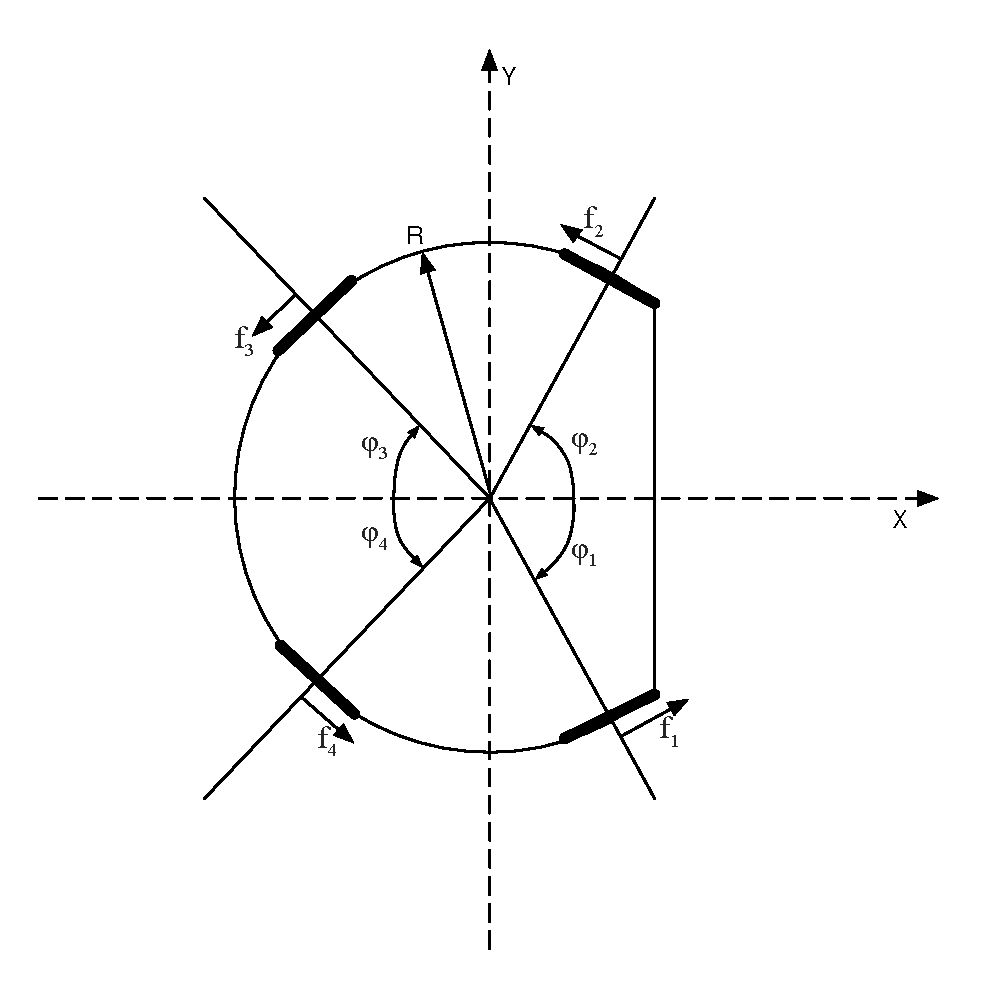
\includegraphics[width=8cm]{anglesRobot.eps}
  \caption{Distribución de Ángulos y Fuerzas}
  \label{fig:angFzaDiag}
\end{figure}
%%%%%%%%%%%%%%%% end figure %%%%%%%%%%%%%%%%%%%
A partir de un movimiento deseado, expresado en el vector de velocidades deseadas \( V_l= \begin{pmatrix} v_x & v_y & \omega \end{pmatrix}^{T} \), es necesario descomponerlo en velocidades de motores deseadas \( V_m= \begin {pmatrix} m_1 & m_2 & m_3 & m_4 \end{pmatrix}^{T} \). 

A partir de la ecuacion general de fuerza Eqn. (\ref{eq:FMA}) se puede derivar la Eqn. (\ref{eq:fmaMots}) específica para el caso de cuatro motores. Debido a las ruedas omnidireccionales, cada motor aporta en los componentes de X y Y. Utilizando el diagrama de la Fig. \ref{fig:angFzaDiag}, es posible derivar la Eqn. ~(\ref{eq:max1}) para el motor 1 en X y Eqn. ~(\ref{eq:may1} para el motor 1 un Y. Similarmente, se pueden obtener las ecuaciones para los otros motores.\par
%%%%%%%%%%%%%%%% Equation %%%%%%%%%%%%%%%%%%
\begin{equation}
  F= Ma \label{eq:FMA} \\
\end{equation}
\begin{equation}
  a = \frac{1}{M}\left(F_1+F_2+F_3+F_4\right) \label{eq:fmaMots} \\
\end{equation}
%%%%%%%%%%%%%% End Equation %%%%%%%%%%%%%%%%
\begin{equation}
  Ma_{1x} = \mid f_1 \mid \cos\left(90 - \varphi_1\right) =  \mid f_1 \mid  \sin\left(\varphi_1\right)\label{eq:max1}
\end{equation}
\begin{equation}
  Ma_{1y} = \mid f_1 \mid \cos\left(\varphi_1\right) \label{eq:may1}
\end{equation}
% \begin{equation}
%   Ma_{2x} = - \mid f_2 \mid  \sin\left(\varphi_2\right)
% \end{equation}
% \begin{equation}
%     Ma_{2y} = \mid f_2 \mid \cos\left(\varphi_2\right) 
% \end{equation}
% \begin{equation}
%   Ma_{3x} = - \mid f_3 \mid  \sin\left(\varphi_3\right)
% \end{equation}
% \begin{equation}
%     Ma_{3y} = \mid f_3 \mid \cos\left(\varphi_3\right)
% \end{equation}
% \begin{equation}
%   Ma_{4x} = \mid f_4 \mid  \sin\left(\varphi_4\right) 
% \end{equation}
% \begin{equation}
%     Ma_{4y} = \mid f_4 \mid \cos\left(\varphi_4\right)  \label{eq:Ma-xy234}\\
% \end{equation}

Para obtener la aceleración angular que aporta cada motor al robot, de la Eqn.~(\ref{eq:omegaGral}) donde R es el radio de acuerdo a la Fig. \ref{fig:ruedaOmni} se puede derivar la Eqn.~(\ref{eq:omega4Mots}) específica para el uso de 4 motores. Sustituyendo el momento de inercia Eqn.~(\ref{eq:inercia}) para el caso de un cilindro con distribución de masa desconocida en (\ref{eq:omega4Mots}) se obtiene la Eqn.~(\ref{eq:Romega}). \par

\begin{equation}
  \dot{\omega} = \frac{Rf}{I} \label{eq:omegaGral} 
\end{equation}
\begin{equation}
  \dot{w} =\frac{R}{I}\left(f_1+f_2+f_3+f_4\right) \label{eq:omega4Mots}
\end{equation}
\begin{equation}
  I = \alpha M R^{2} ;\qquad 0\leq \alpha \leq1 \label{eq:inercia}
\end{equation}
\begin{equation}
  R\dot{\omega} = \frac{1}{M\alpha}\left(f_1+f_2+f_3+f_4\right) \label{eq:Romega}
\end{equation}

A partir de de los resultados obtenidos de las aceleraciones traslacionales y angulares, se puede derivar la Eqn.~(\ref{eq:matAcoFzas}). Tambien se puede expresar como en la Eqn.~(\ref{eq:gralAcoFzas}), donde \( C_\alpha \) se conoce como la Matriz de Acoplamiento de Fuerzas. \par

% Matriz de Acoplamiento de Fuerzas
\begin{equation}
  \left(\begin{array}{c}
    a_x \\ a_y \\R_{\dot{\omega}}
  \end{array}\right)= \frac{1}{M}
  \begin{bmatrix}
    \sin\varphi_1 & -\sin\varphi_2 & -\sin\varphi_3 & \sin\varphi_4 \\
    \cos\varphi_1 & \cos\varphi_2 & -\cos\varphi_3 & -\cos\varphi_4 & \\
    \frac{1}{\alpha} & \frac{1}{\alpha}  & \frac{1}{\alpha}  &\frac{1}{\alpha} 
  \end{bmatrix}
  \left(\begin{array}{c}
    f_1 \\ f_2 \\ f_3 \\ f_4  \label{eq:matAcoFzas}\\ 
  \end{array}\right) 
\end{equation}
\begin{equation}
  a=C_\alpha F \label{eq:gralAcoFzas} \\
\end{equation}

Para poder realizar la transformación de la velocidad deseada en el espacio a velocidades de cada motor, es necesario considerar tanto el perímetro de la rueda como el factor de reducción mediante la Eqn. \eqref{eq:reductorPerim}. A partir de esta, se pueden obtener las ecuaciones de cada motor definiendo el vector \( v_m = \begin{pmatrix}v_1 & v_2 & v_3 & v_4\end{pmatrix} ^{T}\) mediante la Eqn. \eqref{eq:velsMots}  y su forma reducida, la Eqn. \eqref{eq:velsMotsReduce} donde a \( D \) se le conoce como la Matriz de Acoplamiento de Velocidades. \par 

\begin{equation}
  V_{l}^{'} = \frac{ V_l \cdot e } { 2 \pi r} \label{eq:reductorPerim}
\end{equation}
\begin{equation}
  % v_1 = v_x \sin\varphi_1 + v_y\cos\varphi_1 + R \omega \label{eq:velMot1}\\
  v_m = 
    \left(\begin{array}{c}
      v_1 \\ v_2 \\ v_3 \\ v_4 
    \end{array}\right)
    = 
    \begin{bmatrix}
      \sin\varphi_1 & \cos\varphi_1 & 1 \\
      -\sin\varphi_2 & \cos\varphi_2 & 1 \\
      -\sin\varphi_3 & -\cos\varphi_3 & 1 \\
      \sin\varphi_4 & -\cos\varphi_4 & 1 \\
    \end{bmatrix}
    \left(\begin{array}{c}
      v_x^{'}  \\ v_y^{'}  \\ {Rw}^{'} 
    \end{array} \right) \label{eq:velsMots} \\
\end{equation}
\begin{equation}
    v_m = D V_{l}^{'} \label{eq:velsMotsReduce} \\
\end{equation}
\par

% Gracias a la retroalimentación obtenida de cada motor, es posible calcular la velocidad real \( V_{l}^{r} \) a la cual se está moviendo cada motor. Además, es posible determinar la velocidad real del robot. A partir de la ecuación \eqref{eq:velsMotsReduce}, definiendo \( D^{+} \) como la una pseudoinversa de D tal que la identidad \eqref{eq:DsToIdent} se cumple y definiendo el vector \( v_m^{r} = \begin{pmatrix}v_1^{r} & v_2^{r} & v_3^{r} & v_4^{r} \end{pmatrix}^{T} \), se obtiene la identidad \eqref{eq:velsMotToVelsRob}. \par

% \begin{equation}
%   D^{+}D = I_3 \label{eq:DsToIdent}
% \end{equation}
% \begin{equation}
%   V_{l}^{r} = D^{+}v_m \label{eq:velsMotToVelsRob} b
% \end{equation}

% Para el caso específico en el que \(  \varphi_1 = \varphi_2 \) y \(  \varphi_3 = \varphi_4 \), la pseudoinversa es la siguiente:

% \begin{equation}
%   D^{+} = \begin{bmatrix}a & -a &-c & c \\e & e & -g & -g \\ i & i & k & k \end{bmatrix} \\
% \end{equation}
% Donde:
% \begin{equation}
%   \begin{aligned}
%   a & = c \cdot \cos \varphi_1  & \qquad k & = \frac{1}{\frac{2\cos \varphi_3}{\cos \varphi_1} + 2} \\
%   c & = \frac{1}{\frac{2 (\cos \varphi_3)(\sin \varphi_1) }{\cos \varphi_1} + 2\sin\varphi_3} & e & = \frac{1}{2(\cos \varphi_1 + \cos \varphi_3)} \\ 
%   i & = \frac{k \cdot \cos \varphi_3}{\cos \varphi_1} & g & = e \\
%   \end{aligned}
% \end{equation}
%%%%%%%%%%%%%%%%%%%%%%%%%%%%%%%%%%%%%%%%%%%%%%%%%%%%%%%%%%%%%%%%%%%%%%
%%%%%%%%%%%%%%%% begin figure %%%%%%%%%%%%%%%%%%%
\begin{figure}
  \centering
    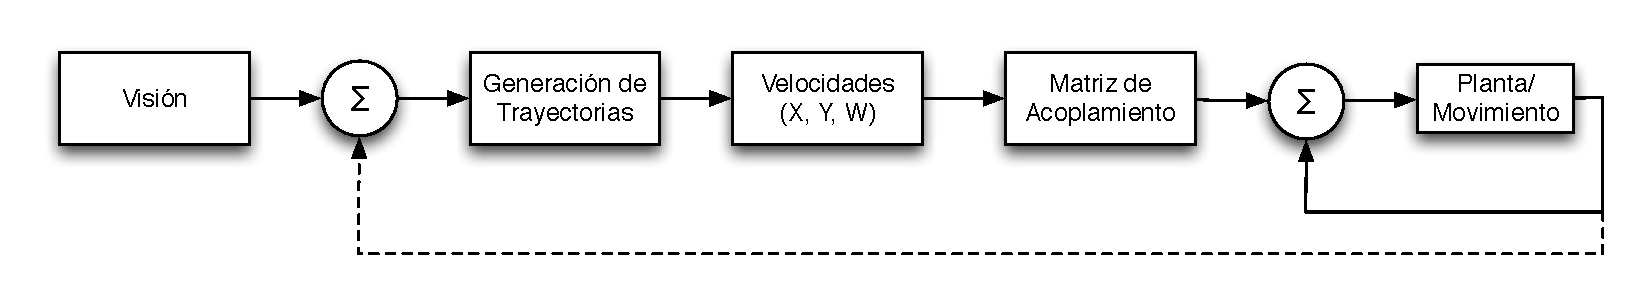
\includegraphics[width=8cm]{esquema_PID_motor.eps}
  \caption{Esquema de Control Implementado}
  \label{fig:ctrl}
\end{figure}
%%%%%%%%%%%%%%%% end figure %%%%%%%%%%%%%%%%%%% 
%%%%%%%%%%%%%%%%%%%%%%%%%%%%%%%%%%%%%%%%%%%%%%%%%%%%%%%%%%%%%%%%%%%%%%
\subsection*{CONTROL}
Para el control a bajo nivel, se utiliza la retroalimentación que otorga cada motor, implementando un control PI a nivel motor. El esquema general del algoritmo de control utilizado se muestra en la Fig. \ref{fig:ctrl}. La sintonización de las variables se realiza a mano siguiendo el método de Ziegler - Nicholson. \par
% Se incorporó un PI a nivel motor, utilizando el método de Ziegler - Nicholson para realizar la sintonización de las variables.
Adicional al control PI por motor, se cuenta con la retroalimentación de la visión gracias a la cual se puede calcular y corregir la trayectoria del robot al enviar continuamente actualizaciones de la velocidad deseada (30 Hz). 
% En la Fig. \ref{fig:visionPrueba} se muestran las trayectorias seguidas por el robot al utilizar solamente el control PI así como utilizando el control PI y la retroalimentción de la visión.

%%%%%%%%%%%%%%%%%%%%%%%%%%%%%%%%%%%%%%%%%%%%%%%%%%%%%%%%%%%%%%%%%%%%%%
%%%%%%%%%%%%%%%% begin figure %%%%%%%%%%%%%%%%%%%
\begin{figure}
  \centering
    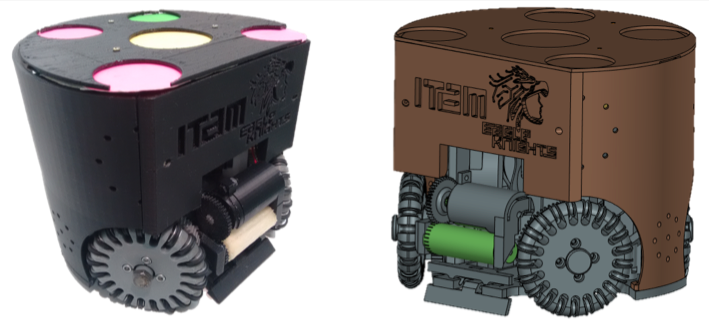
\includegraphics[width=8cm]{realVS3D.png}
  \caption{Robot Real vs Modelo 3D del Robot}
  \label{fig:ModRealVSdes}
\end{figure}
%%%%%%%%%%%%%%%% end figure %%%%%%%%%%%%%%%%%%% 
%%%%%%%%%%%%%%%%%%%%%%%%%%%%%%%%%%%%%%%%%%%%%%%%%%%%%%%%%%%%%%%%%%%%%%
\section*{RESULTADOS}
Con el diseño propuesto se logra que el robot se mueva aproximadamente a la velocidad propuesta, manteniendo la integridad de sus componentes y con un peso menor que el contemplado inicialmente, aunque siendo capaz de cargar los 3.5 Kg propuestos. Tanto la carcasa como la base y las ruedas han sido capaces de resistir golpes entre los robots a las velocidades normales de movimiento y la visión reconoce el patrón estandar incoporado en la carcasa. En la Fig. \ref{fig:ModRealVSdes} se muestra una comparación entre el diseño modelado en 3D y la construcción final del robot.\par 
En la Fig. \ref{fig:realVSdes} se puede ver la respuesta de un motor ante una velocidad deseada con el algoritmo de control PI implementado. Aunque las oscilaciones no se eliminan, se reducen rápidamente, siendo la respuesta rápida uno de los factores más importantes debido al dinamismo del sistema. Igualmente, el motor es capaz de cambiar de velocidad, incluso a velocidades negativas (dirección contraria) rápidamente. \par
Estableciendo 8 direcciones en el plano XY, se probó la respuesta del robot ante cada direccion con control PI sin visión y con visión. En la Fig. \ref{fig:visionPruebasRetro} se pueden ver los resultados de estas pruebas.Para el caso del robot sin retroalimentación de visión, existen algunas direcciones en las cuales el movimiento y su posición final es cercano al deseado, especificamente en las direcciones en que practiamente no se utilizan dos ruedas. En cambio en las otras direcciones, se tiene mayor error en el movimiento del robot. Para el caso del movimiento con retroalimentación de visión, aunque en algunos casos existe un movimiento errático, la posición final es muy cercana a la deseada gracias a la correción que realiza el sistema ante los errores en el movimiento del robot. \par

%%%%%%%%%%%%%%%%%%%%%%%%%%%%%%%%%%%%%%%%%%%%%%%%%%%%%%%%%%%%%%%%%%%%%%
%%%%%%%%%%%%%%%% begin figure %%%%%%%%%%%%%%%%%%%
\begin{figure}
  \centering
    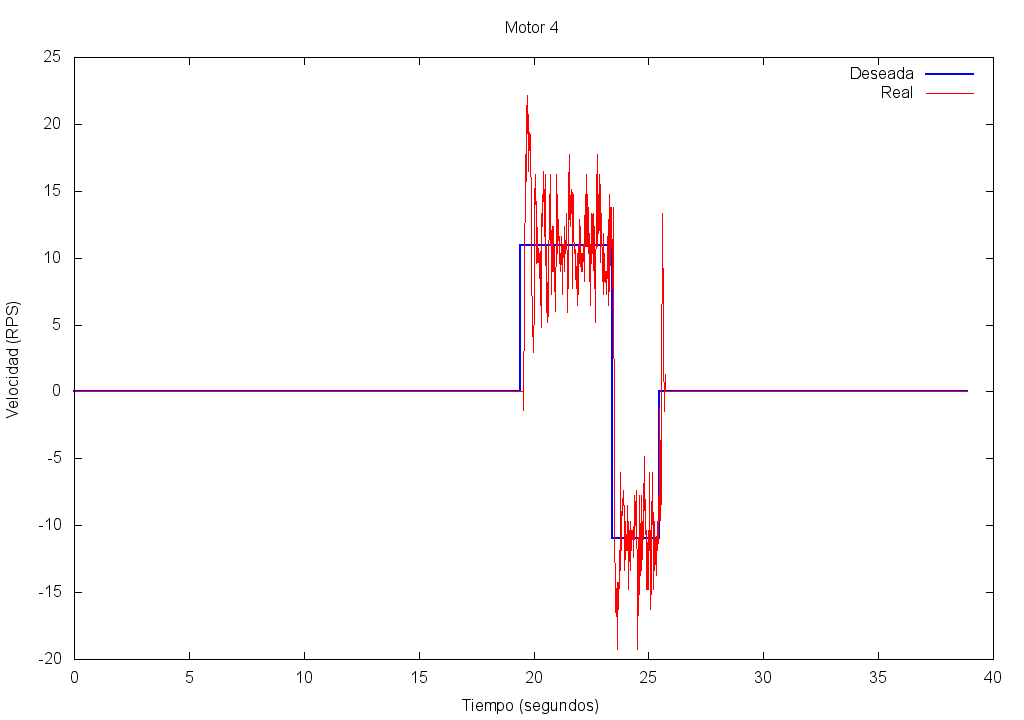
\includegraphics[width=8cm]{VelocidadM4.png}
  \caption{Velocidad real vs Velocidad deseada}
  \label{fig:realVSdes}
\end{figure}
\begin{figure}
  \centering
    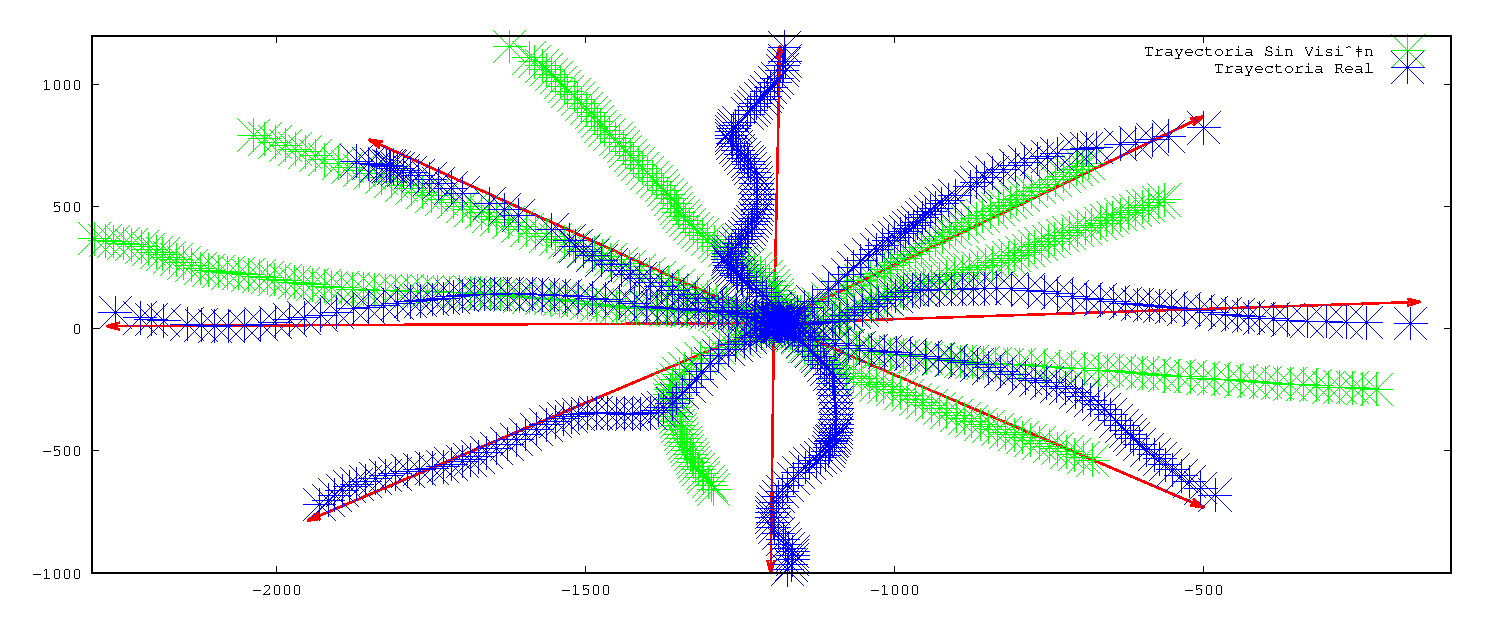
\includegraphics[width=8cm]{output1.eps}
  \caption{Trayectorias con retroalimentación}
  \label{fig:visionPruebasRetro}
\end{figure}
%%%%%%%%%%%%%%%% end figure %%%%%%%%%%%%%%%%%%% 


%%%%%%%%%%%%%%%%%%%%%%%%%%%%%%%%%%%%%%%%%%%%%%%%%%%%%%%%%%%%%%%%%%%%%%


%%%%%%%%%%%%%%%%%%%%%%%%%%%%%%%%%%%%%%%%%%%%%%%%%%%%%%%%%%%%%%%%%%%%%%
%%%%%%%%%%%%%%% begin table   %%%%%%%%%%%%%%%%%%%%%%%%%%
% \begin{table}[t]
% \caption{THE TABLE CAPTION USES CAPITAL LETTERS, TOO.}
% \begin{center}
% \label{table_AMRob}
% \begin{tabular}{c l l}
% & & \\ % put some space after the caption
% \hline
% Example & Time & Cost \\
% \hline
% 1 & 12.5 & \$1,000 \\
% 2 & 24 & \$2,000 \\
% \hline
% \end{tabular}
% \end{center}
% \end{table}
%%%%%%%%%%%%%%%% end table %%%%%%%%%%%%%%%%%%% 
%%%%%%%%%%%%%%%%%%%%%%%%%%%%%%%%%%%%%%%%%%%%%%%%%%%%%%%%%%%%%%%%%%%%%%

% All tables should be numbered consecutively and  captioned; the caption should use all capital letters, and centered above the table as shown in Table~\ref{table_AMRob}. The body of the table should be no smaller than 7 pt.  There should be a minimum two line spaces between tables and text.

%%%%%%%%%%%%%%%%%%%%%%%%%%%%%%%%%%%%%%%%%%%%%%%%%%%%%%%%%%%%%%%%%%%%%%
\section*{CONCLUSIÓN}
La construcción del robot cumple con las especificaciones establecidas en las reglas F180. El movimiento del robot es correcto y se puede patear y utilizar el \textit{dribbler}. El algoritmo de control funciona correctamente aunque es posible realizar una mejor sintonización. Se cuenta con la arquitectura general del sistema, pudiendo ir agregando nodos y modificandolos de ser necesario. \par
Como trabajo futuro se propone un método de sintonización automático para el sistema de control. Adicionalmente, es necesario implementar un algoritmo de evación de obstáculos así como de especificar tareas para cada uno de los robots del equipo. \par


% \section*{FOOTNOTES\protect\footnotemark}
% \footnotetext{Examine the input file, asme2e.tex, to see how a footnote is given in a head.}

% Footnotes are referenced with superscript numerals and are numbered consecutively from 1 to the end of the paper\footnote{Avoid footnotes if at all possible.}. Footnotes should appear at the bottom of the column in which they are referenced.


%%%%%%%%%%%%%%%%%%%%%%%%%%%%%%%%%%%%%%%%%%%%%%%%%%%%%%%%%%%%%%%%%%%%%%
% \section*{CITING REFERENCES}

%%%%%%%%%%%%%%%%%%%%%%%%%%%%%%%%%%%%%%%%%%%%%%%%%%%%%%%%%%%%%%%%%%%%%%
% The AMRob reference format is defined in the authors kit provided by the AMRob.  The format is:

% \begin{quotation}
% {\em Text Citation}. Within the text, references should be cited in  numerical order 
% according to their order of appearance.  The numbered reference citation should be 
% enclosed in brackets.
% \end{quotation}

% The references must appear in the paper in the order that they were cited.  In addition, 
% multiple citations (3 or more in the same brackets) must appear as a `` [1-3]''.

% The bibliography style required by the AMRob is unsorted with entries appearing in the 
% order in which the citations appear. If that were the only specification, the standard 
% {\sc Bib}\TeX\ unsrt bibliography style could be used. Unfortunately, the bibliography 
% style required by the ASME has additional requirements (last name followed by first 
% name, periodical volume in boldface, periodical number inside parentheses, etc.) that 
% are not part of the unsrt style. Therefore, to get ASME bibliography formatting, you 
% must use the \verb+amrob.bst+ bibliography style file with {\sc Bib}\TeX. This file is 
% not part of the standard BibTeX distribution so you'll need to place the file someplace 
% where LaTeX can find it (one possibility is in the same location as the file being typeset).


% Here's where you specify the bibliography style file.
% The full file name for the bibliography style file 
% used for an ASME paper is asmems4.bst.
\bibliographystyle{amrob.bst}


%%%%%%%%%%%%%%%%%%%%%%%%%%%%%%%%%%%%%%%%%%%%%%%%%%%%%%%%%%%%%%%%%%%%%%
\begin{acknowledgment}
Gracias al Instituto Tecnológico Autónomo de México, específicamente al departamento de Sistemas Digitales por el apoyo brindado al Laboratorio de Robótica. 
\end{acknowledgment}

%%%%%%%%%%%%%%%%%%%%%%%%%%%%%%%%%%%%%%%%%%%%%%%%%%%%%%%%%%%%%%%%%%%%%%
% The bibliography is stored in an external database file
% in the BibTeX format (file_name.bib).  The bibliography is
% created by the following command and it will appear in this
% position in the document. You may, of course, create your
% own bibliography by using thebibliography environment as in
%
% \begin{thebibliography}{12}
% % ...
% \bibitem{itemreference} D. E. Knudsen.
% {\em 1966 World Bnus Almanac.}
% {Permafrost Press, Novosibirsk.}
% % ...
% \end{thebibliography}

% Here's where you specify the bibliography database file.
% The full file name of the bibliography database for this
% article is asme2e.bib. The name for your database is up
% to you.
\bibliography{amrob.bib}

%%%%%%%%%%%%%%%%%%%%%%%%%%%%%%%%%%%%%%%%%%%%%%%%%%%%%%%%%%%%%%%%%%%%%%
\appendix       %%% starting appendix
% \section*{Appendix A: Head of First Appendix}
% Avoid Appendices if possible.

%%%%%%%%%%%%%%%%%%%%%%%%%%%%%%%%%%%%%%%%%%%%%%%%%%%%%%%%%%%%%%%%%%%%%%
% \section*{Appendix B: Head of Second Appendix}
% \subsection*{Subsection head in appendix}
% The equation counter is not reset in an appendix and the numbers will
% follow one continual sequence from the beginning of the article to the very end as shown in the following example.
% \begin{equation}
% a = b + c.
% \end{equation}

\end{document}
